\newpage\sloppy
% \setlength{\RaggedRightHyphenpenalty}{500}
\setlength{\RaggedRightRightskip}{0pt plus 2em}
\section{สถาปัตยกรรมองค์กร (TOGAF)}

TOGAF (The Open Group Architecture Framework) คือกรอบแนวคิดมาตรฐานสำหรับ การออกแบบและบริหารจัดการสถาปัตยกรรมองค์กร ซึ่งให้หลักการวิธีการและเครื่องมือที่เป็นระบบ ในการพัฒนาสถาปัตยกรรมที่สอดคล้องกับวัตถุประสงค์ทางธุรกิจ

\begin{center}
	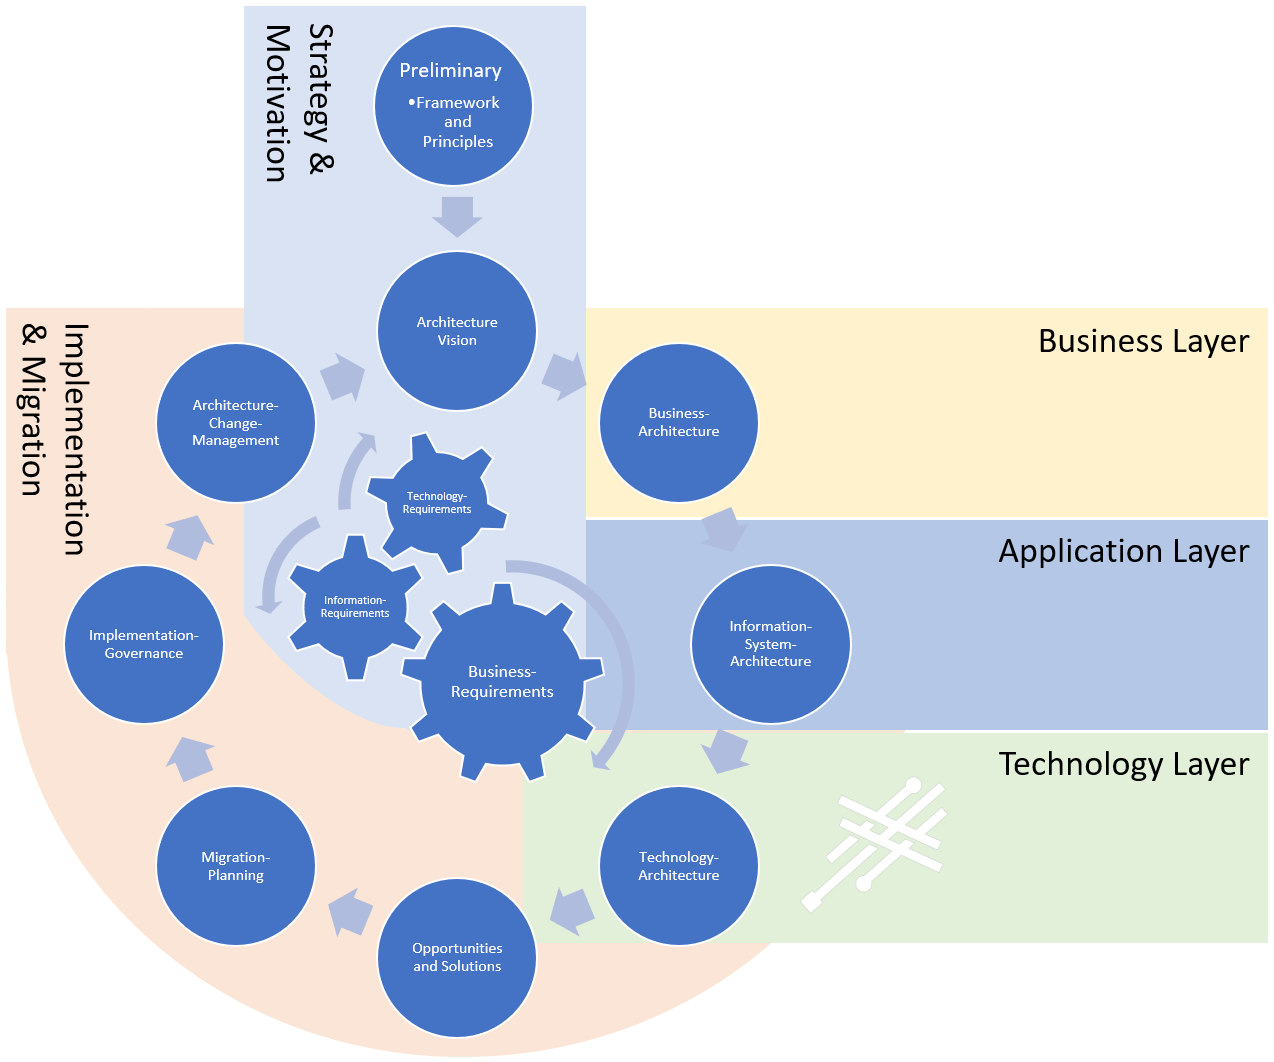
\includegraphics[width=0.9\textwidth]{figures/ea-diagram.png}
\end{center}

\textbf{เหตุผลที่เลือกใช้ TOGAF:}
\begin{itemize}
    \item \textbf{มาตรฐานสากล:} เป็นกรอบแนวคิดที่ได้รับการยอมรับอย่างกว้างขวางจากองค์กรทั่วโลก
    \item \textbf{ความยืดหยุ่น:} สามารถปรับใช้ได้กับองค์กรขนาดใหญ่และขนาดเล็ก
    \item \textbf{การจัดการวงจรชีวิต:} มีแนวทางชัดเจนสำหรับการพัฒนาและปฏิบัติการสถาปัตยกรรม
    \item \textbf{การสื่อสารระหว่างทีม:} ใช้โมเดล ArchIT ซึ่งเป็นเครื่องมือมาตรฐานสำหรับการกำกับดูแลและตรวจสอบสถาปัตยกรรมองค์กร
\end{itemize}

\fussy
